%% ====================================================================
\chapterwithtoc{Introduction}
\label{chapter:verification}
%% ====================================================================

Computers have been used for variety of applications in business, science, education, engineering and so on. They help to solve real world problems that would otherwise be slow, impossible or extremely difficult to address without computers and software. However, sometimes they do not behave exactly as we expect them to do. In some cases, the consequence could be very serious for errors in banking systems
and flight control systems. Errors in computer systems are mostly not caused by the machine itself, but typically originate from the software that controls the computer systems, so called bugs. 
%% ********************************************************************
\KW{Complex machines}%
%% ********************************************************************
Bugs are quite common in complex software systems,
since they typically have complicated input and involve many features which makes them difficult to design and make them perfect by human effort.
%% ********************************************************************
\KW{Find bugs}%
%% ********************************************************************
Detecting and fixing software bugs are important tasks in software development process. Remaining undetected bugs in any software project may lead huge
problems. They can be very hard to detect and correct. It will
become too costly to solve. Therefore, it is very important to allocate sufficient
resources, both in terms of time and manpower, to ensuring that developed
software is as free of bugs as possible.

%% ********************************************************************
\KW{Safety$\Rightarrow$no bugs}%
\index{Critical systems}%
\index{Safety}%
%% ********************************************************************

Some bugs are less serious than others. In some cases, we can still use software programs with these bugs. For example, bugs appearing in computer games and online news. However, in the case of critical systems 
%such as banking, software systems in airplanes, safety is the most important aspect and we have to ensure that there no bugs in either the software nor the hardware.
especially algorithms in libraries of programming languages, safety is the most important aspect and we have to ensure that there no bugs. These algorithms are used in many applications, and bugs will have wide impacts. Some of such libraries provide standard data structures such as stacks, queues, containers. These data structures provide ways of storing multiple values in a single variable.

A data structure is a particular way of organizing and storing data in a computer so that it can be accessed and modified efficiently. More precisely, a data structure is a collection of data values, the relationships among them, and operations that can be applied to the data. 
%Each data structure has it own specification which describes the behaviour of the data structure. 
A data structure can be both sequential or concurrent, concurrent data structures can be accessed and manipulated concurrently by many parallel threads are a central component of many parallel software applications. 
%They should allow a large degree of parallelism among accessing threads to minimize serialization bottlenecks, while maintaining the appearance of atomic operations. 
Data structures typically use heap-allocated memory to store their data. For example, concurrent link queue in java.util.concurrent uses singly linked list data structure to store data.   


%Many modern programming languages provide libraries of concurrent data structures (e.g., the java.util.concurrent package and Intel Threading Building Blocks library) that are widely used. 



The predominant method to improve software quality is
\emph{testing}. It is a dynamic analysis where a program is run under specific conditions, so-called test cases, and checking
whether the result with a given input matches the expected output.
%
The test cases are carefully designed to cover all possible cases of program executions.\index{Coverage}
%% ********************************************************************
\KW{Simulation}\index{Verification Methods!Simulation}%
%% ********************************************************************
%Similarly, we can check for correctness of a program by using a \emph{model} of the program. The model can be extracted by
%removing all parts that are irrelevant for the tests, and can be used
%to \emph{simulate} the executions. 
However, there is no guarantee to cover all possible executions. Therefore, we have to find the way to achieve a full coverage of program executions. \emph{testing} can be used to show the presence of bugs, but never to show their absence. So, it is needed to use formal verification that a software system is correct with respect to some specifications. %
%
% The topic of this thesis is centered around the following question.
% %
% \begin{statement}
%   \it%
%   Can we design a method that would give us\\%
%   \emph{guarantees} that no error is left undetected\\%
%   and that does not (too much) suffer from state-space explosion?
% \end{statement}

%\index{Error-free Guarantee}%
%The topic of this thesis is design methods guaranteeing that no error is undetected and that do not suffer from state-space explosion.

%% ====================================================================
\section*{Formal Verification} 
%Computer programs are written based on human intuition, which is probably leads to programming errors. Current practice is to test programs on various sample inputs in the hope of finding any possibility of incorrect program behavior. There exist many approaches like testing, simulation, static analysis and simple debugging techniques, such as inserting assertions and print statements in the source code, which show the presence of software errors. 

%Formal verification uses mathematical methods to verify whether a software satisfies its specification provided by users. 
%formal verification is the process of checking whether a software satisfies its predefined properties. 
Formal verification uses mathematical methods to check whether a software satisfies its specification provided by users. 
%formal verification is the process of checking whether a software satisfies its predefined properties. 
%\bjcom{Skip the following sentece. Continue into the next paragraph}
%There is a wide variety of specification to be checked for software programs, these specification can be very domain-specific, as in “train collisions and derailments do not occur in train traffic” or it may be generic, as in “no execution of the system dereferences a null pointer.” 
% be either safety or liveness properties. Liveness properties state that program execution eventually reaches several desirable states at some point of execution, for example liveness properties can be "the postman delivers the letter to the recipient", "A sent message is eventually received". In contract, verifying safety property of a program is satisfied is reduced to checking that something bad will never happen in the execution of the program [48]. 
%\input model
%In order to specify liveness properties, it is needed to  describe traces of events by using temporal logics, statistics, and probabilities. Checking aliveness property is done by repeatedly checking reachability of good situations in program executions. 
There are several approaches for formal verification, including equivalence checking, theorem proving, and model checking. Equivalence checking method decides whether a system is equivalent to its specification with respect to some notion of behavioral equivalence. This is \bjcom{Insert a sentence about where it is used. I think it is mostly used for hardware designs in industry} Theorem proving is a technique where both the \bjcom{insert ``behavior of the''} system and its desired properties are expressed in mathematicaal logic. Then, theorem proving \bjcom{insert ``typically assisted by an interactive theorem prover} will try to prove that the system satisfies these properties. 

Model checking approach take \bjfix{Model checking approach take}{Model checking takes as input} a model of the system under
consideration and a formal specification of the \bjfix{the}{a} property to be verified as inputs. \bjcom{Insert a sentence saying like ``The specification of a software component may consist of a number of such properties, each of which can be verified using model checking''}
The approach exhaustively explorer \bjcor{explores} all possible states  \bjcor{executions} of the model \bjcom{En the sentence here, and start a new one with ``This is typically done exploring the set of reachable states of the model''}  which can be finite or infinite \bjcom{Stop the sentence here, the stuff about infinite and abstraction comes later. Instead, start here by saying that this works well if the set of reachable states is finite, and also say in which application domains this has been successful} where infinite sets of states can be represented finitely by using abstraction techniques. In this way, it can be shown that a given system model truly satisfies a certain specification. Model checking is a general verification approach that is applicable to a wide range of applications
  such as embedded systems, software engineering, \bjcom{Skip ``software engineering''} and hardware design. However, it usually work well with finite-state systems. It is a real challenge to examine the largest possible state spaces that can be treated. For example, applying model checking to infinite-state systems such as data structures with many dimensions of infiniteness is a real challenge in current software verification research.
  \bjcom{The preceding paragraph needs better structure. You can use the flow: what is model checking - it works well for finite-state, e.g., for controllers and hardware design - most software is infinite-state, e.g., a data structure may contain an unbounded amount of data - a common technique for handling this is to devise a symbolic representation of sets of states, such that a single symbolic representation may represent an infinite set of states. Thereafter you can give an overview of
  what has been achieved using symbolic techniques}
%In this thesis though, we consider programs where the specification describes the bad behaviors. We concentrate on safety properties and try to design abstraction techniques to verify that a program including both sequential and concurrent program respects its specifications. 

%\section*{Verification of Data Structures}
%Most modern programming languages provide libraries of data structures such as the C++ Standard Template Library, the Java Collections Framework. A data structure is a particular way of organizing and storing data in a computer so that it can be accessed and modified efficiently. More precisely, a data structure is a collection of data values, the relationships among them, and operations that can be applied to the data. Each data structure has it own specification which describes the behaviour of the data structure. A data structure can be both sequential or concurrent, concurrent data structures can be accessed and manipulated concurrently by many parallel threads are a central component of many parallel software applications. They should allow a large degree of parallelism among accessing threads to minimize serialization bottlenecks, while maintaining the appearance of atomic operations. Many modern programming languages provide libraries of concurrent data structures (e.g., the java.util.concurrent package and Intel Threading Building Blocks library) that are widely used. 
%
%To ensure that a concurrent data structure is correct, we have to ensure that it respects to its sequential specification.  Ideally, the correctness is captured by linearizability. Linearizability is generally accepted as the standard correctness criterion for such concurrent data structure implementations. It states that each operation on the concurrent data structure can be viewed as being performed atomically at some point (called linearization point (LP)) between its invocation and return. The linearizability guarantee relieves the programmer from complex reasoning about possible interference among data-structure methods and removes the need to add explicit synchronization. Concurrent implementations of abstract data structures (stacks, queues, sets, etc.) are becoming more and more complex as implementations that increase the degree of concurrency are identified. This in turn is making linearizability verification harder. Existing approaches lack generality as they are limited to specific classes of concurrent data structures so far no technique (manual or automatic) for proving linearizability has been proposed that is both sound and generic. In this thesis, we focus on verifying safety properties including linearizability of both sequential and concurrent data structures.
\section*{Research Challenges}
%In this thesis, we consider two challenges in software verification, the first challenge is to automate its application to sequential programs that manipulate complex dynamic linked data structures. The problem becomes even more challenging when program correctness depends on relationships between data values that are stored in the dynamically allocated structures. Such ordering relations on data are central for the operation of many data structures such as search trees, priority queues (based, e.g., on skip lists), key-value stores, or for the correctness of programs that perform sorting and searching, etc. The challenge for automated verification of such programs is to handle both 
%\begin{challenges}
%\item infinite sets of reachable heap configurations and
%\item relationships between data values embedded in such graphs, 	
%\end{challenges}
%e.g., to establish sortedness properties, there exist many automated verification techniques, based on different kinds of logics, automata, graphs, or grammars, that handle these pointer structures. Most of these approaches abstract from properties of data stored in dynamically allocated memory cells. The few approaches that can automatically reason about data properties are often limited to specific classes of structures, mostly singly-linked lists (SLLs), and/or are not fully
%automated.
%
%We present a general framework for verifying programs with complex dynamic linked data structures whose correctness depends on relations between the stored data values. Our framework is based on the notion of forest automata (FA) which has previously been developed for representing sets of reachable configurations of programs
%with complex dynamic linked data structures [?]
\bjcom{Start by saying what is the overall challenge of your thesis. Then say that this requires to address several challenges in model checking}
In this thesis, we consider challenges in developing techniques for automated verification of both sequential and concurrent data structures using heaps. 
%Our challenges are to automate its application to both sequential and concurrent programs that manipulate complex dynamic linked data structures. We have to deal with concurrent programs with an unbounded number of threads that concurrently access and manipulate a dynamically allocated shared heap where data stored in each heap cell can be in unbound domain. Such programs and algorithms are difficult to get correct and verify, since their shapes are complicated to represent and they typically employ fine-grained synchronization, replacing locks by atomic operations such as compare-and-swap, and are therefore notoriously difficult to get correct, witnessed. It is therefore important to develop efficient techniques for automatically verifying their correctness. This requires overcoming several challenges. This thesis presents simple and efficient techniques to verify that a concurrent implementation of a common data type abstraction, namely queue, stack, set, conforms to a simple abstract specification of its (sequential) functionality. The data structures we consider for these programs can be singly-linked lists, sets of linked lists or skip-lists. In order to deal with this problem, we have to deal with several combined challenges as follow.
We have to deal with several sub-challenges as following: 
\bjcom{I suggest to use more standard bullets. Each bullet can have a number of letter, and have a heading of a few words, e.g, {\bf Dynamically heap-allocated memoty}. Also, do not just break the page here}
\bjcom{Each challenge should be described better. You must be more precise in what cannot be done with current techniques, and (on an abstract level) what you
  will try to achieve}
\newpage
\begin{challenges}
\item Heaps which are used by data structures are dynamically heap allocated memory. Therefore, we have to deal with unbounded number of heap cells. In this thesis, we propose three heap abstraction techniques to address the challenge, including forest automata, summary abstraction and view abstraction.
\item In each cell of a heap, the domain of data values can be unbounded. We use the combination of shape analysis and data abstraction to deal with this challenge. 
  \bjcom{I suggest to start with this challenge (since it is the first paper). You can start the preceding text and simplify it. The important aspect is that there
    are current approachs for heaps and for data, but not for combining them in suitable ways, and thereafter you describe very briefly your approach. Here is
    the disappeared text: ``In this thesis, we consider two challenges in software verification, the first challenge is to automate its application to sequential programs that manipulate complex dynamic linked data structures. The problem becomes even more challenging when program correctness depends on relationships between data values that are stored in the dynamically allocated structures. Such ordering relations on data are central for the operation of many data structures such as search trees, priority queues (based, e.g., on skip lists), key-value stores, or for the correctness of programs that perform sorting and searching, etc. The challenge for automated verification of such programs is to handle both 
\begin{itemize}
\item infinite sets of reachable heap configurations and
\item relationships between data values embedded in such graphs, 	
\end{itemize}
e.g., to establish sortedness properties, there exist many automated verification techniques, based on different kinds of logics, automata, graphs, or grammars, that handle these pointer structures. Most of these approaches abstract from properties of data stored in dynamically allocated memory cells. The few approaches that can automatically reason about data properties are often limited to specific classes of structures, mostly singly-linked lists (SLLs), and/or are not fully
automated''}

We present a general framework for verifying programs with complex dynamic linked data structures whose correctness depends on relations between the stored data values. Our framework is based on the notion of forest automata (FA) which has previously been developed for representing sets of reachable configurations of programs
with complex dynamic linked data structures [?]

\item We have to verify that the data structures are correct with any number of threads that access and manipulate the structures. We use the thread modular technique to dead with this challenge.
\item \bjcom{This paragraph should be improved. I suggest to make it the second challenge. You can start by saying that for concurrent data structures, you address
  a number of challenges, and then you have three bullets for each of them. The first is how to specify correctness in a way that is suitable for automated verification, the second is how to deal with an unbounded number of threads, the third is to provide a simple shape abstraction which can express relevant properties of different classes of heap structures: You can talk about skiplists, and their challenges}
To ensure that a concurrent data structure is correct, we have to ensure that it respects to its sequential specification.  Ideally, the correctness is captured by linearizability. Linearizability is generally accepted as the standard correctness criterion for such concurrent data structure implementations. It states that each operation on the concurrent data structure can be viewed as being performed atomically at some point (called linearization point (LP)) between its invocation and return. The linearizability guarantee relieves the programmer from complex reasoning about possible interference among data-structure methods and removes the need to add explicit synchronization. Concurrent implementations of abstract data structures (stacks, queues, sets, etc.) are becoming more and more complex as implementations that increase the degree of concurrency are identified. This in turn is making linearizability verification harder. Existing approaches lack generality as they are limited to specific classes of concurrent data structures so far no technique (manual or automatic) for proving linearizability has been proposed that is both sound and generic. In this thesis we provide a sound and generic technique to verify linearizabilities of concurrent data structures.
\item In some data structures, the each cell can have unbound number of pointer field such as cells in skip-lists and arrays of lists. This problem is solved by our fragment abstraction technique.
\end{challenges}

\bjcom{The outline must be more complete.}
We present, in the next chapters, the general background about model checking, concurrent data structures. Thereafter, in the following chapter, we introduce in a stepwise manner how
we cope with  above challenges. In the last chapter, we summary and give future plans for our work.

%% ====================================================================
\chapter{Model Checking}
\label{section:model:checking}
\index{Model Checking}%
\index{Verification Methods!Model Checking}%
%% ====================================================================
%
% Within the field of formal verification, 
The approach that we focus on this thesis is
\emph{model-checking}.
%% ********************************************************************
\KW{Automation}%
\index{Automation}%
%% ********************************************************************
This method will try to verify whether a model of the program
satisfies its specification.
%
%It is often called a push-button technology.
%
 
This approach was introduced by Emerson and Clarke~\cite{CE82} and by Queille and Sifakis~\cite{QS82}. The method requires a model of the system under
consideration and a property as input. The method then computes and returns either "correct" when the specification is satisfied by the program, or "incorrect" when the program does not satisfy its specification. In the case of incorrect answer, the method can explain the reason by giving a counter-example. A state in the model contains relevant information about the program. Alongside all the states of the system, the model depicts the
transitions, i.e.\ how to move from one state to another state. Every behaviour of the system is represented as a succession of transitions, starting from some initial states. States and transitions together describe the \emph{operational
  semantics}, that is, how every step of the system takes place in the model. The number of states and transitions can be finite or infinite. Model-checking aims to explore the state-space entirely from some initial states. However, when the state-space is of large size. It grows in-fact
exponentially with the number of parameters or the size of their
domain. Therefore, there have been several methods to address with the
state-space explosion problem.
%\begin{figure}[h]
%{\noindent\centering %
%  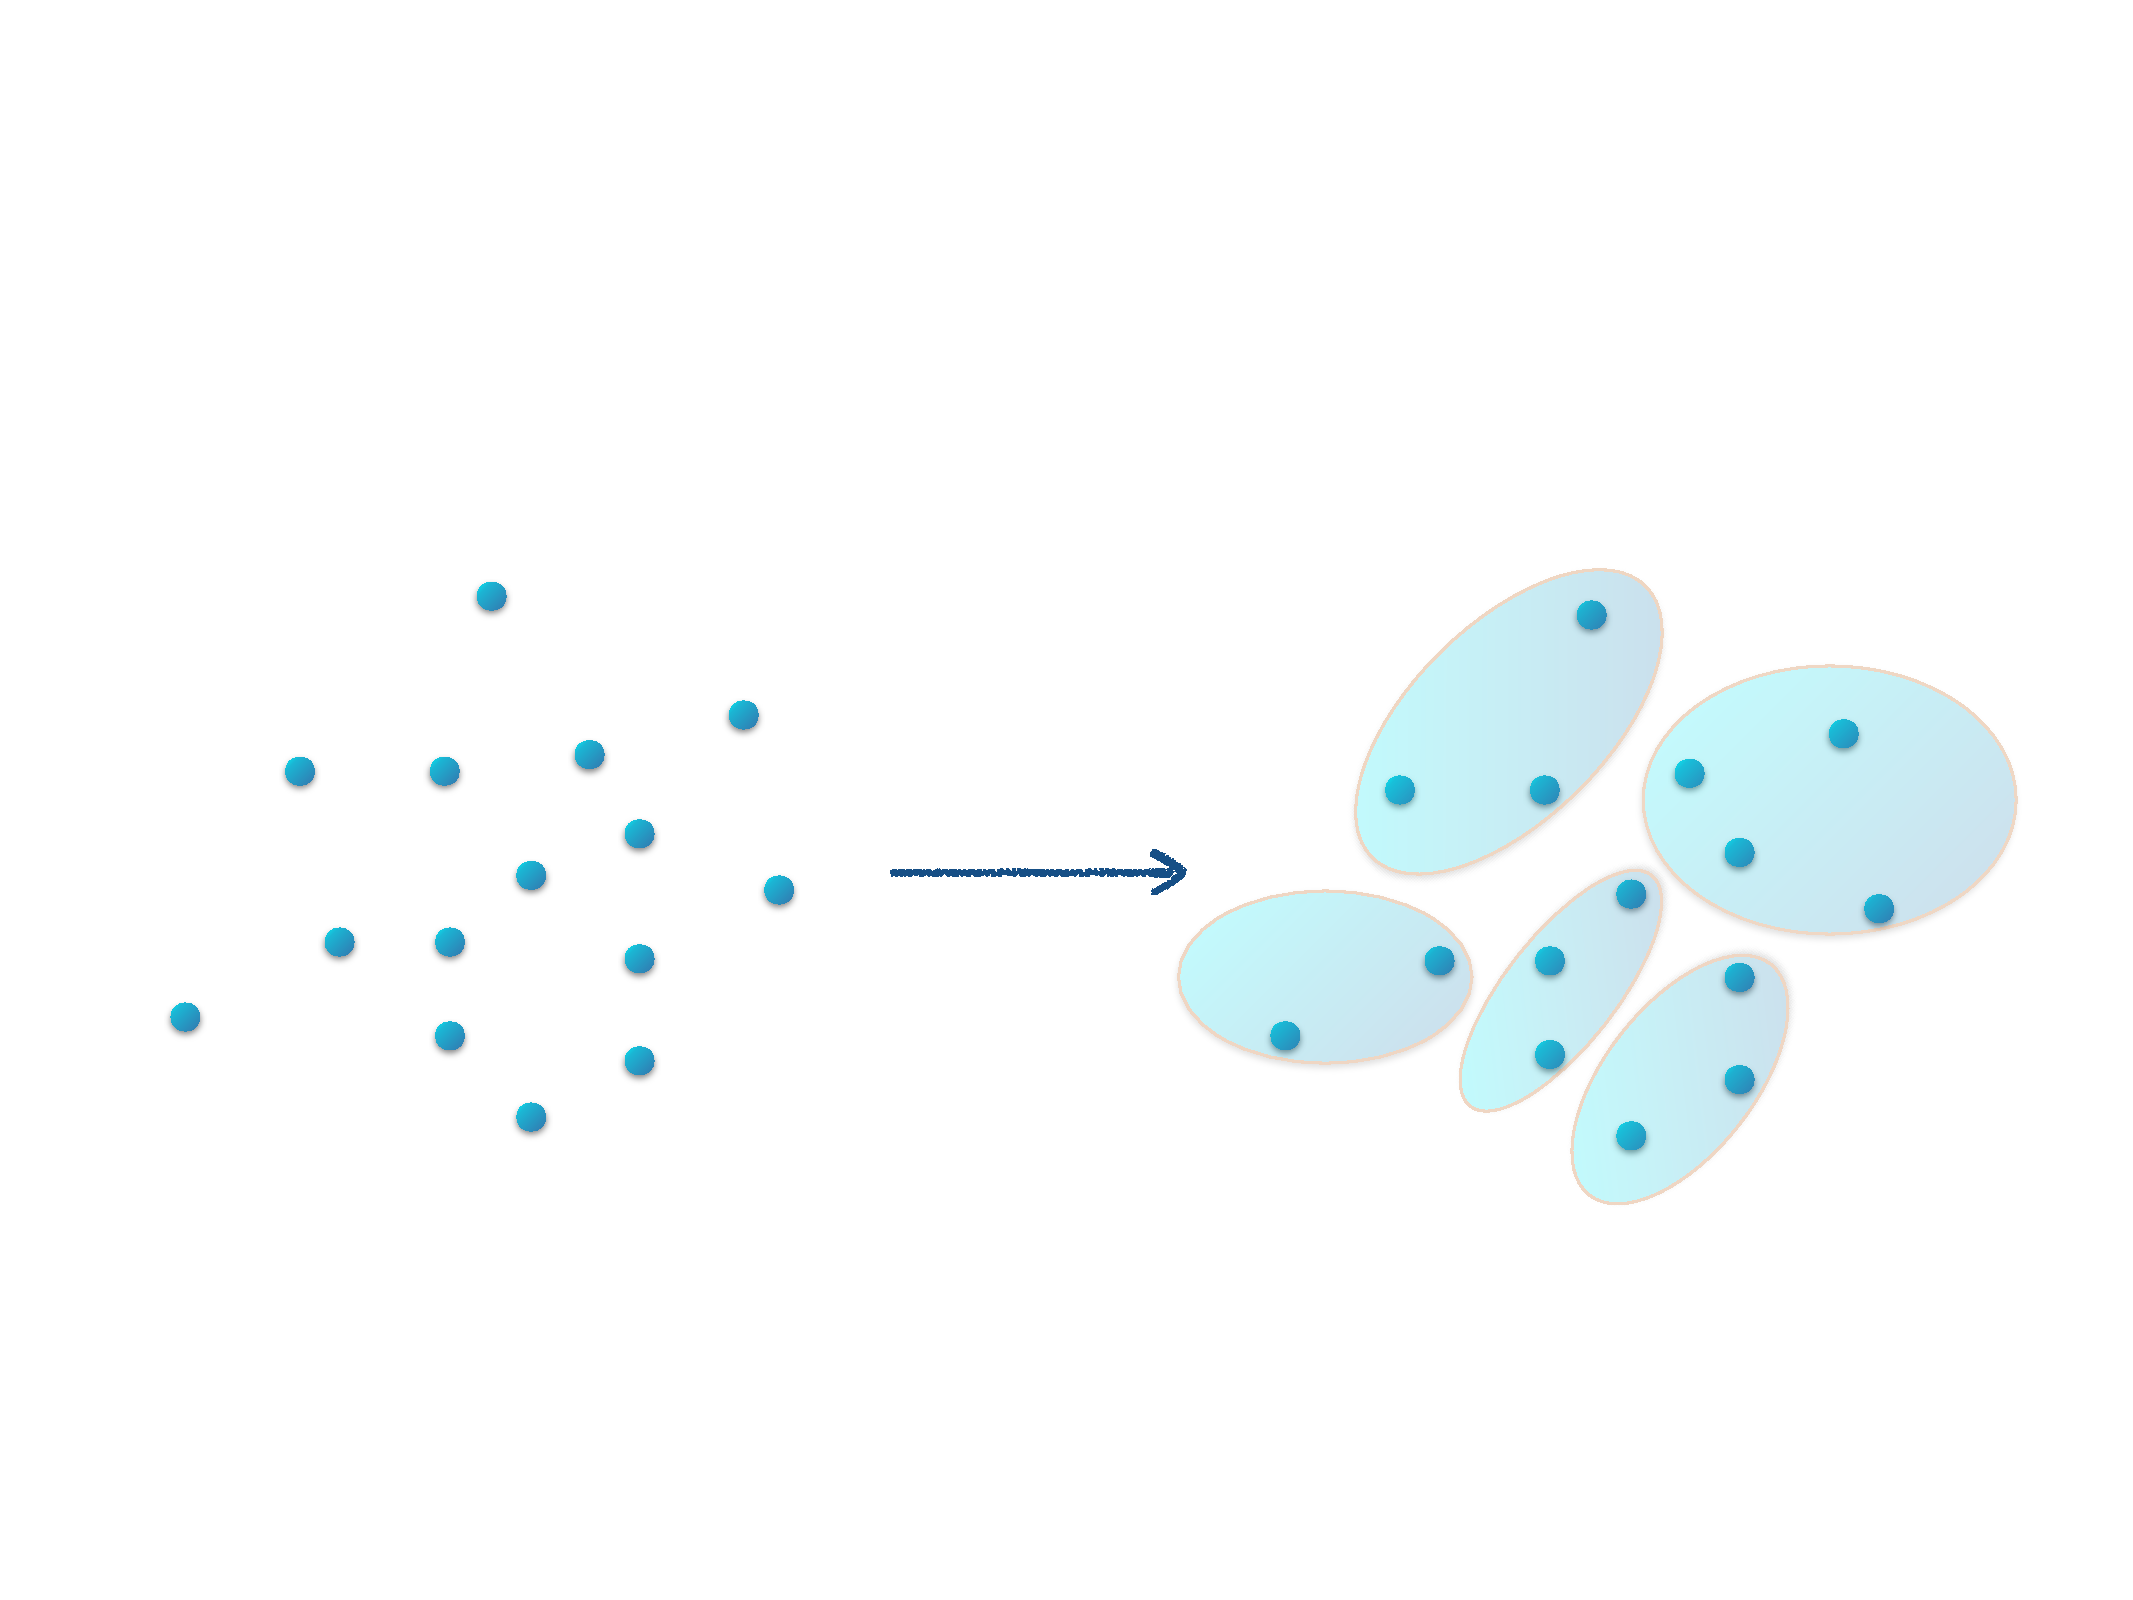
\includegraphics[trim=4cm 4cm 1.5cm 2cm,clip,scale = 0.3]{img/modelchecking.pdf}%
%  \par%
%}%
%\caption{Example of symbolic representation where the right part is a concrete reachable state-space and the left part is abstract state-space using symbolic representation}
%\label{symbolicabs}
%\end{figure}
%\vspace{1cm}
%\begin{figure}[h]
%  \centering
%  \tikzinput{img/symbolic-representations}    
%  \vspace{0.3cm}
%  \caption{Symbolic Representation}      
%\label{symbolicabs}
%\end{figure}
%\vspace{1cm}
                   
There are several techniques addressing the state-space explosion problem.
The choice of which transition to pick during the exploration can be
crucial for the efficiency of the procedure. In some cases, exploring all orderings of events is not necessary because some states can be re-visited. \emph{Partial order} techniques aim at detecting and avoiding
redundant situations, while retaining important dependencies among
actions. They however do not reduce the state-space. The main approach called \emph{symbolic
  representation}  to solve the state-space explosion problem is to avoid representing concretely all states of the system. The process is performed by designing abstract states so that each abstract state could represent a set of concrete states.  This designing process is done by \emph{dropping} irrelevant details based on properties that we want to verify. For example, consider a switch with two positions: {\tt up} and {\tt down}. The switch has a counter that indicates how many times the light was turn on. Initially, its position is {\tt down}, the light is {\tt off} and the counter is $\tt 0$. When the switch is shifted up, the light is turned on, and the counter is incremented by $\tt 1$. When we shift the switch down, the light is turned off and the counter is reset to $\tt 0$ if it had reached its maximum value. We want to verify that the switch can not be up and the light is off at the same time. If we keep all the information of the system, then, a state consists of the position of the switch, the status of the light and the value of the counter, we would have $\tt (2*2*n)$ states where $\tt n$ is the maximum value of counter. If $\tt n$ is $\tt 1000000$ then we may end up to four million states.  However, it is obvious that the counter is not needed to verify the property, so we could ignore it then a state contains only the position and status of the switch and the light denoted as $\tt [p,s]$ where $\tt p$ is the position and $\tt s$ is the state of the light. The system using the symbolic representation moves from  [{\tt down;off}]  to  [{\tt up;on}]  and conversely from  [{\tt up;on}]  to  [{\tt down;off}] . We see that the state-space exploration never visits a state that belongs to the set labeled by  [{\tt down;on}]  therefore the system is safe. The switch example is of course simple and does not reflect the complexity of today’s software. Symbolic representations are of crucial help to combat the state-space explosion, accelerate the algorithms and get them to terminate in a reasonable amount of time

%By doing that, we get an set of abstract states from reachable states of a concrete system. Thereafter, the method returns safe if the abstract states do not contain any bad state. The approach described in figure \ref{symbolicmodelchecking}.  %
%
The challenge is to find over-approximations that do not introduce
behaviours that could turn out to be bad. Indeed, the method would
return that the property is not satisfied and we would not know
whether it comes from the approximation or from the concrete system
itself. % 
                                   
%\begin{figure}
%{\noindent\centering %
%  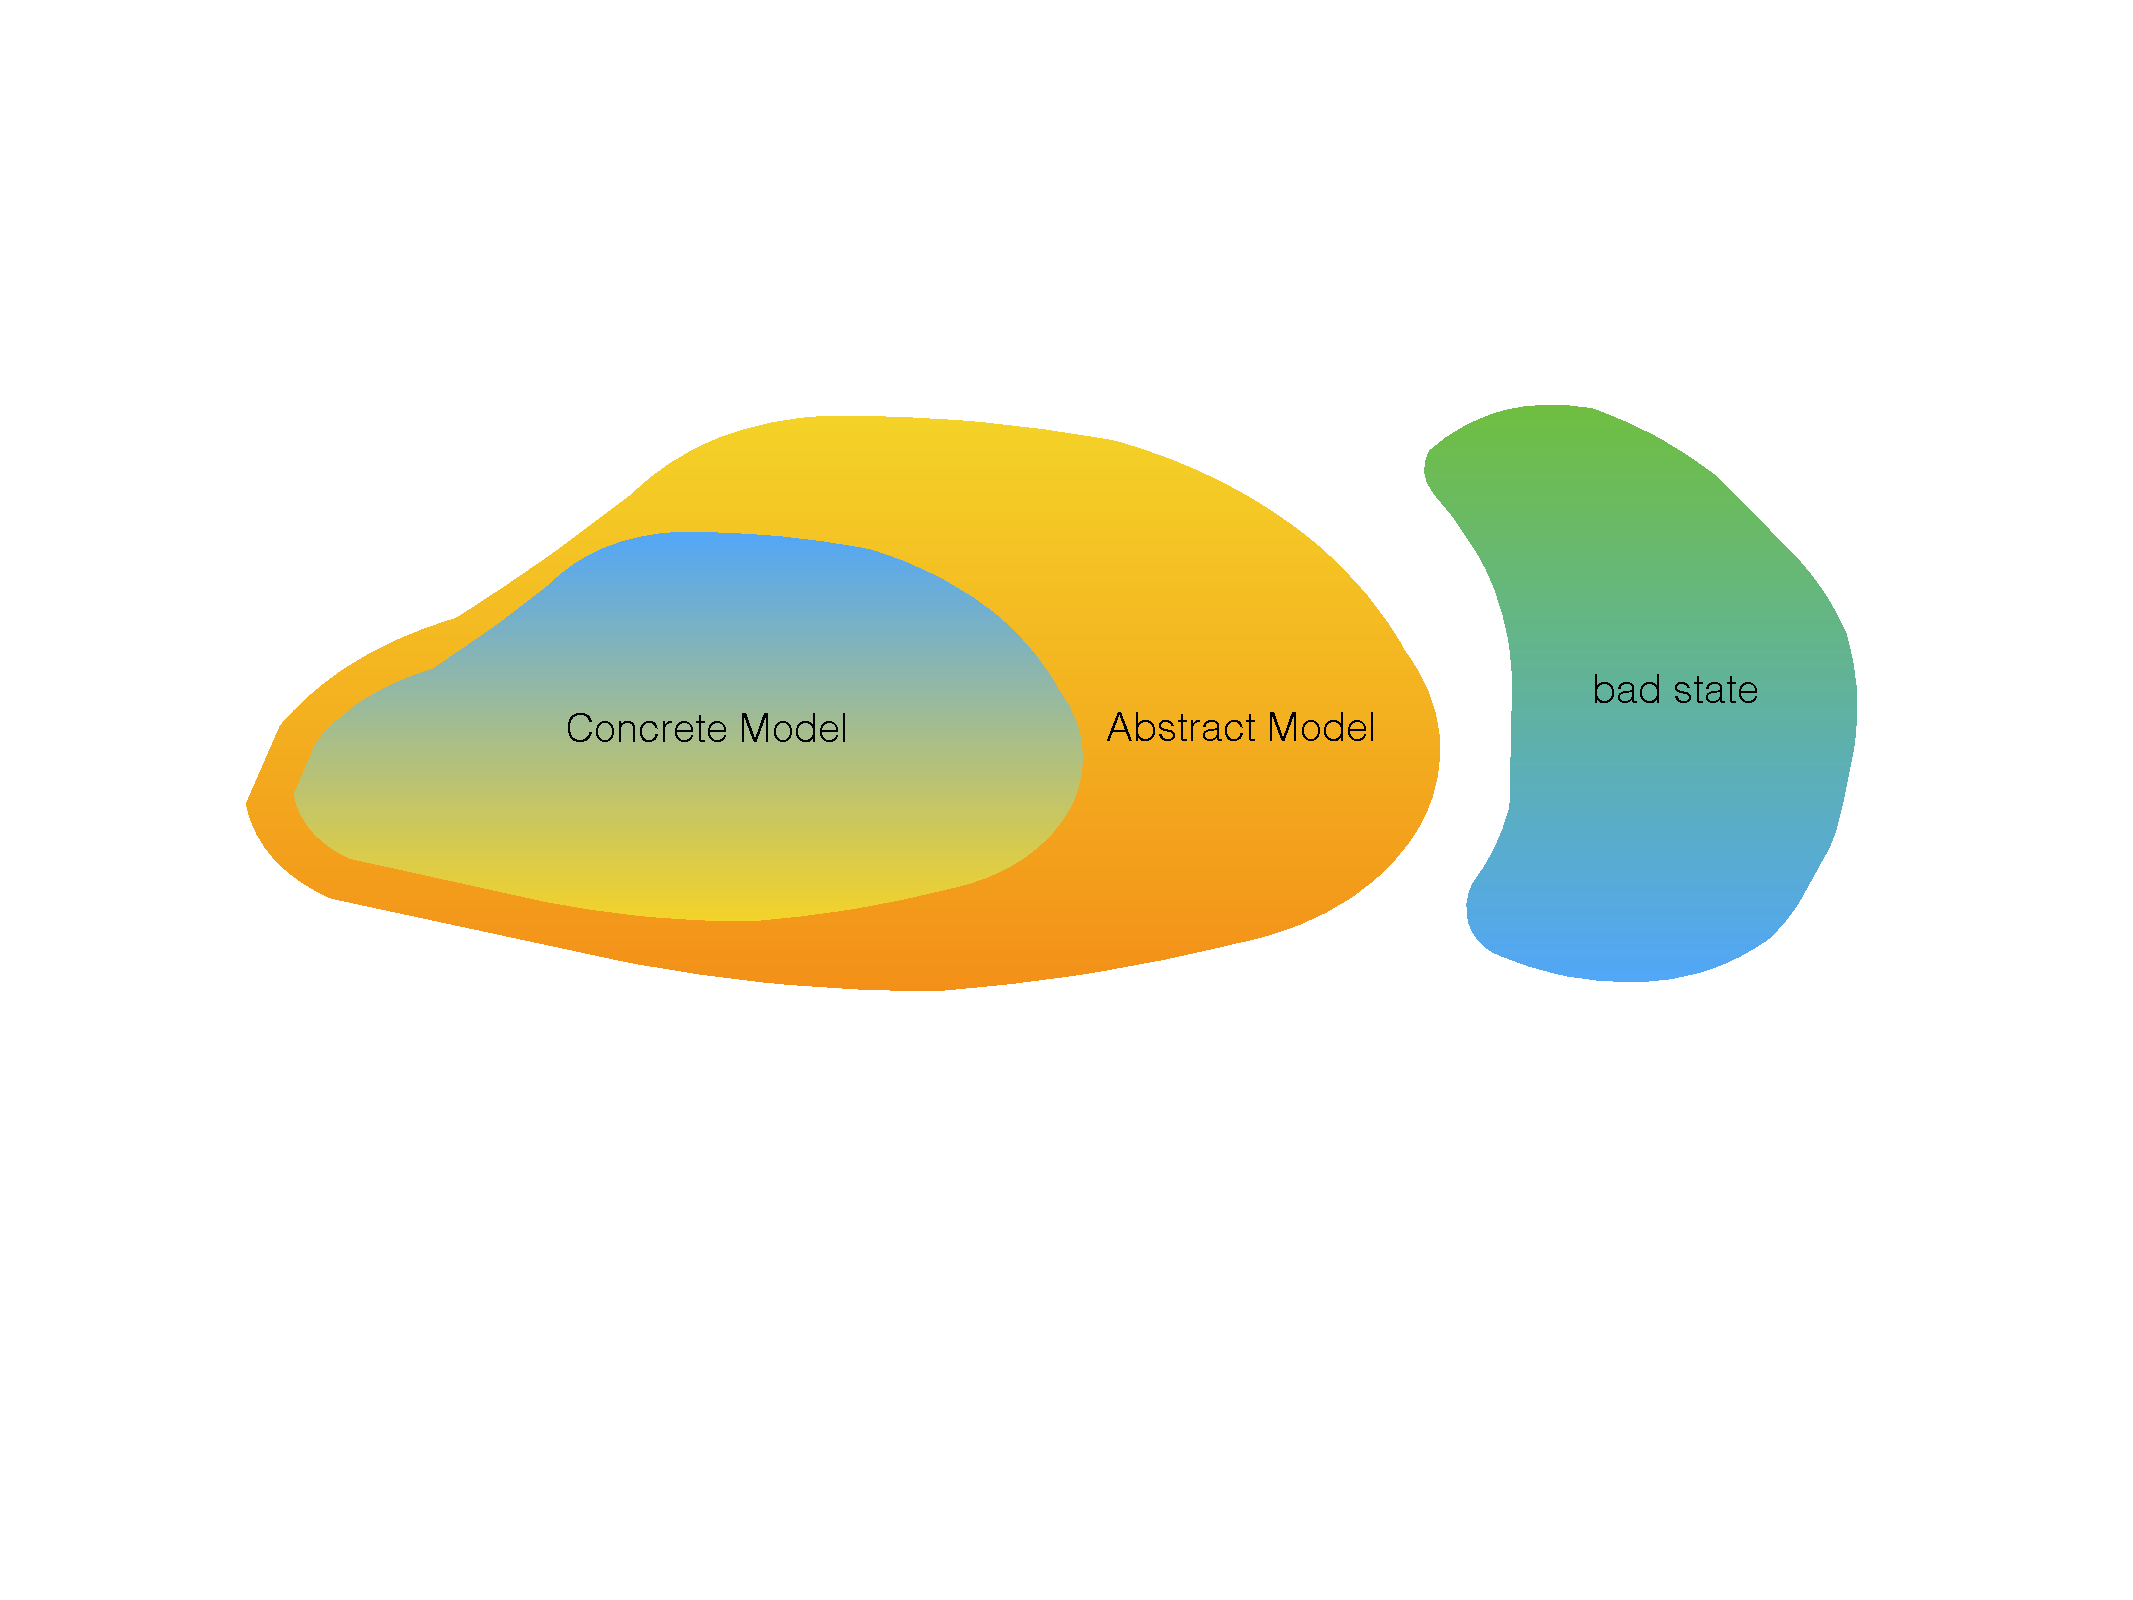
\includegraphics[trim=0cm 6cm 2cm 2cm,clip,scale = 0.25]{img/badstate.pdf}%
%  \par%
%}%
%\caption{Symbolic model checking architecture }	
%\label{symbolicmodelchecking}
%\end{figure}


%\vspace{1cm}
%\begin{figure}[h]
%  \centering
%  \tikzinput{img/approximations} 
%  \vspace{0.3cm}
%\caption{Symbolic model checking architecture }	
%\label{symbolicmodelchecking}
%\end{figure}
%\vspace{1cm}

To palliate to the imprecision caused by a too coarse
over-approximation, it is possible to analyze the returned
counter-example and find the origin of the problem. If it turns out to
be a real concrete example, the method has in fact found a bug, and
the property is surely not satisfied. Otherwise, the counter-example
comes from the approximation, that is, there is a step in the sequence
of events leading to that counter-example which is not performed by
the original system but only by the abstract model. The approximation
is be refined by discarding this step and the method should be run
anew.

Nevertheless, finding suitable over-approximations is a challenge on
its own. %
This thesis now revolves around the following problem statement.
%
%\begin{statement}
%  {\bf Safety}: %
%  {\it Given a specification and an (over-)approximation,\\does the
%    abstract system reach a bad configuration?}
%\end{statement}
%

%%%% ====================================================================
%\section{Parameterized Verification}
%\label{section:paramsys}
%%% ====================================================================
%\KW{Parameter-ized systems are infinite-state}%
%\index{Parameterized Systems}%
%%% ********************************************************************
%Many systems can actually be characterized as a family of finite-state
%systems with one (or more) parameter ranging over an unbounded domain.
%%
%For each fixed value of the parameter, the system is finite-state.
%%
%However, a system that contains an \emph{a priori} unknown parameter
%must behave properly regardless of the value of the parameter. It is
%therefore considered infinite-state.
%
%%% ********************************************************************
%\KW{Parameter-ized verification}%
%\index{Parameterized Verification}%
%%% ********************************************************************
%The \emph{parameterized verification} problem is to prove
%correctness %\footnote{\ldots and namely here safety only}
%of the system, against some specification, for all values of the
%parameter.
%%
%For example, in the case of a program manipulating a list, the
%parameter could be the length of the list. The system as a whole is a
%set of finite-state systems, one for each length of the list.
%%
%For a network protocol, the parameter could be the topology of the
%network and the system is to be proven safe regardless of how the
%network nodes are arranged.
%
%%% ********************************************************************
%\KW{Parameter-ized systems}%
%%% ********************************************************************
%We concentrate in this thesis on a specific class of
%\emph{parameterized systems}, namely, systems consisting of an
%arbitrary number of processes (see
%Chapter~\ref{chapter:parameterized:systems}). %
%The size of the system is the parameter of the verification problem.
%% 
%For each value $n$ of the parameter, the system $S_n$ is the parallel
%composition of $n$ processes, which can interact with each other at
%any time.
%%
%\index{Safety}%
%Given a specification, we prove safety for the family $(S_n)_{n\ge 0}$
%--- as~a~whole --- by showing the non-reachability of some
%(potentially infinite) set of \emph{bad states}. %
%%
%We use the following strategy:
%\begin{strategy}
%\item \index{Model}%
%  We extract a model from each process in the system. This in turn
%  defines the operational semantics with states and transitions for
%  the entire family.
%\item \index{Over-approximation}%
%  We use an over-approximation to derive an abstract model from the
%  original (infinite-state) model.  This defines a new state-space and
%  set of transitions.
%\item \index{Abstract Model}%
%  We determine two sets in the abstract model:
%  \begin{itemize}[itemsep=0pt, leftmargin=0cm]
%    % \item the initial states --- usually mirroring the initial settings
%    %   of the program,
%  \item \index{Initial states}%
%    the initial states, usually mirroring the initial settings of the
%    program,
%    % \item the bad states --- usually along the lines of the targeted
%    %   property.
%  \item \index{Bad states}%
%    the bad states, usually along the lines of the targeted property.
%  \end{itemize}
%\item \index{Reachability}%
%  We finally check whether the bad states are reachable from the
%  initial states in the abstract model.
%  % 
%  % \item Apply model-checking techniques (from
%  %   Chapter~\ref{chapter:monotonic:abstraction}~or~\ref{chapter:view:abstraction})
%  %   to determine wether the bad states are reachable from the initial
%  %   states, by following a sequence of transitions --- also known as the
%  %   reachability problem.
%\end{strategy}%
%%
%\index{Soundness}%
%By construction of the over-approximation, showing that the abstract
%model is safe, will imply that the original system is also correct
%with respect to its specification, regardless of the number of
%processes in the system.
%%
%We present a formal definition and some examples in the next chapter.
%
%%% ********************************************************************
%\newpage
%\subsection*{Heap analysis}
%\KW{Heaps}%
%\index{Heap Analysis}%
%%% ********************************************************************
%An important extension in this thesis is the application of
%parameterized verification to the complex problem of shape analysis.
%%
%We consider programs that implement data-structures that can be
%concurrently accessed by an arbitrary number of threads.
%%
%The data-structures, e.g.\ stacks and queues, are constructed using
%singly-linked lists.
%%
%By following the chains of pointers, we observe that programs leave
%memory footprints that we coin \emph{shapes} or \emph{heaps}.
%
%The number of threads is one dimension of the parametrization. 
%%
%Shape analysis can also be parameterized along other dimensions, such
%as the size of the data-structure or the data domain.
%%
%In Chapter~\ref{chapter:shape:analysis}, we address the combined
%challenges of an arbitrary number of threads, an unbounded size of
%heaps and an unbounded data domain. Moreover, we do not assume the
%presence of a garbage collector which makes the task even more
%complex.
%
%The program specification itself is infinite since the programs can
%manipulate data values from a domain of unbounded size.
%%
%It is not enough to inspect each shape and conclude that it belongs to
%a particular set of bad shapes. We need to observe \emph{traces} of
%events. We therefore pair each shape with a special \emph{observer}
%whose role is to determine whether a sequence of events might not
%occur for a particular data-structure.
%%
%We still apply the above-described strategy and conclude that the
%program reaches a bad configuration when the observer is in a bad
%state.
%%
%We dedicate Chapter~\ref{chapter:shape:analysis} to explain this
%complex problem and the verification method in further details.

\newpage
%%%% ====================================================================
%\section[Theoretical Limitations \ldots\ \emph{not}!]{Theoretical Limitations}
%\KW{Decidability}%
%\KW{Theoretical limitations}%
%\index{Theoretical limitations}%
%%% ====================================================================
%It is important to understand the type of programs that the methods
%can handle and with which limitations.
%%
%\index{Theoretical limitations!Decidability}%
%A problem is %said
%\emph{decidable} if there exists an algorithm to solve \emph{every}
%instance of the problem.
%% Otherwise, it is \emph{undecidable},
%% which is also the case when some instances can be solved but not all.
%%
%% Even though undecidable problems are hard ones to solve, some
%% instances can potentially still be solved.
%\index{Theoretical limitations!Intractability}%
%Decidable problems can still be \emph{intractable}, that is, even if a
%solution exists, it is difficult to compute because it requires too
%much time or space resources.
%%
%On the contrary, in the case of undecidable problems, it is sometimes
%possible to design algorithms that can work well in practice for
%\emph{some} instances but do not guarantee to compute a solution for
%all input combinations or even terminate in general.
%%
%Research challenges regarding the theoretical limitations of
%algorithms consist of identifying %
%(i) undecidable problems and %
%(ii) classes of systems and specifications for which the verification
%problem is decidable and designing efficient algorithms for these.
%%
%
%% The verification problem is known to be undecidable in general, but
%% decidable for the subclass of parameterized systems which are well
%% quasi-ordered
%% (WQO)~\cite{Parosh:Bengt:Karlis:Tsay:general,abdulla:well}.
%The problem of parameterized verification is well-known to be
%undecidable in general~\cite{Parosh:Bengt:Karlis:Tsay:general} %
%but for some subclass of systems (see
%Chapters~\ref{chapter:monotonic:abstraction}
%to~\ref{chapter:shape:analysis}), the verification problem becomes
%decidable, yet complex, and we present efficient algorithms to solve
%it.
%% chapter~\ref{chapter:monotonic:abstraction},
%% \ref{chapter:view:abstraction} and~\ref{chapter:shape:analysis}.
%%
%
%We would like to pinpoint that this thesis is \emph{not} about
%theoretical results on decidability of some class of programs.
%%
%Rather than providing computational bounds on the time and/or amount
%of space in memory the verification algorithms require or comparing
%which algorithm is best, the thesis focuses %instead
%%on whether the algorithms are practical. %
%on finding the suitable abstractions that make the algorithms
%\emph{practical}, i.e.\ terminate in a reasonable amount of time.
%% In other words, do they compute the answers in a reasonable amount of
%% time?
%We shall not bother much about the amount of space they require,
%because we can assume that %, as long as it stays within reason,
%it is always possible to extend the capacity of the machine and re-run
%the methods. %
%
%In the coming chapters, we will describe the different techniques to
%make the algorithms usable in practice. This was the challenge and we
%present the results in this thesis.
%%
%\begin{statement}
%  \it%
%  This focus of this thesis is on designing efficient algorithms\\%
%  for the intractable problem of parameterized verification\\%
%  for a specific class of programs.
%\end{statement}
%
%% There are numerous methods targeting primarily WQO systems and proven
%% to be complete for them. %
%% Universally quantified transitions are not monotonic, and systems with
%% such transitions are not WQO. %
%% Some of these methods are however still sound for such systems, and
%% were successfully used to verify many of them, mostly because these
%% systems have an inductive and upward-closed invariant which is strong
%% enough to imply safety. %
%% The WQO specialized methods are bound to fail, if they cannot derive
%% such upward-closed invariants.
%% %
%% Refer to Section~\ref{section:related_work} for more details on
%% related works.


%% ====================================================================
%\whatwelearned{verification}
%% ====================================================================
